\documentclass[a4paper,11pt]{article}
\usepackage[utf8]{inputenc}

\usepackage{geometry}
\usepackage{graphicx}
\usepackage{hyperref}
\usepackage[table]{xcolor}

\definecolor{dgreen}{rgb}{0.1,0.6,0.1}  %zielony


\geometry{hmargin={2cm, 2cm}, height=10.0in}
%nowy typ kolumny o zadanej szerokosci + wycentrowanej
\newcolumntype{C}[1]{>{\centering\arraybackslash}p{#1}}



% Title Page
\title{Efficiency and purity determination of the particle identification method in the Central Exclusive Production process for the STAR experiment at RHIC\\[12pt]\large Project for the Python in the Enterprise by T.Szumlak\vspace{-10pt}}
\author{Łukasz Fulek, Rafał Sikora\vspace{-10pt}}
\date{September 13, 2016}


\begin{document}
\maketitle

\begin{abstract}
This is the report explaining basic concepts and features of the program prepared as an assesment project for the Python in the Enterprise, implemented under python in version 2.7. It contains description of all components of the program and short discussion of the results of analysis, which this program was intended to enable.
\end{abstract}

\section{Project objectives}

The main (initial) goal of our project, whose name was ``Machine learning – particle identification (PID) for the STAR experiment using neural net approach'', was to develop an algorithm which would use a machine learning to enhance efficiency and purity of particle identification in the STAR experiment at RHIC in a specific class of particle reactions called ``diffractive interactions''. In this class of interactions STAR detector does not provide an information about the time of collision, because no particles are produced in the mid-forward region (pseudorapidity $\eta$ of approximately 4-5), and therefore standard procedure of reconstruction of inversed particle velocity $\beta^{-1}$ can not be applied (for more detailed explanation see~\cite{1}).

Because of a few reasons we decided to partially change the topic of our project. First, we have received recommendations from the physics working group (PWG) in the STAR experiment to postpone development of the machine learning PID, because such approach is not widely used in other STAR analyses and usage of such would be problematic in terms of review of paper proposal in the future.
Second, experiment have some difficulties with the detector geometry implementation in the GEANT3 environment and thus production of Monte Carlo (MC) samples with detector response simulation is not possible at the moment, therefore it would be helpful to have some evaluation of currently used PID method.

Given facts above the goal of our project was set to write a toy-MC generator simulating the detector response for the case of exclusive production of two oppositely charged particles, and determine the efficiency and purity of the ``nominal'' particle identification procedure.

\section{Particle identification method}
\begin{figure}[ht]
  \centering
  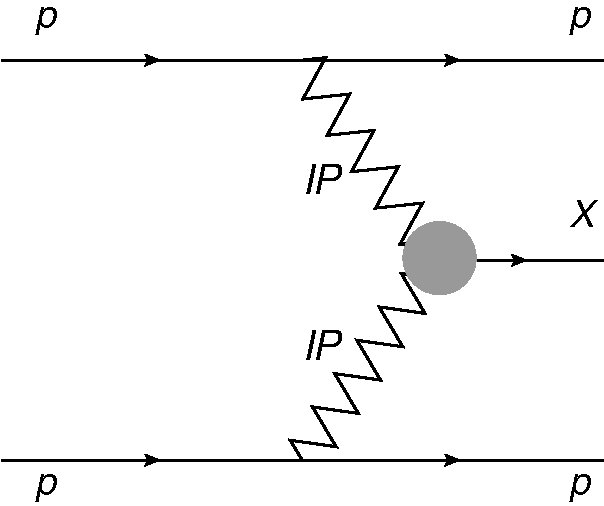
\includegraphics[width=0.3\textwidth]{graphics/DPE.pdf}
  \caption{Feynman diagram of Double Pomeron Exchange process.}
   \label{fig:DPE}
\end{figure}

In the case of Central Exclusive Production process, which at high center-of-mass energies occurs mostly via the Double Pomeron Exchange (Fig.~\ref{fig:DPE}), in the mid-rapidity region neutral state $X$ is produced, which then decays dominantly into a pair of opposite-charge particles, e.g. $\pi^{+}\pi^{-}$. In the analysis of this process we use reconstructed observables from the STAR detector such as track length, track momentum, track energy loss dE/dx (all three from the Time Projection Chamber (TPC)) and time of hit detection in the barrel Time-Of-Flight (TOF) system. The two-particle event is schematically presented in Fig.~\ref{fig:TofSketch}.

In the nominal PID method, whose evaluation has been performed with the help of prepared python program, we use the so called nSigma variables, defined as
\begin{equation}
n\sigma_{Y} = \log{\frac{\textrm{d}E/\textrm{d}x_{\textrm{measured}}}{\textrm{d}E/\textrm{d}x_{~Y,\textrm{Bichsel}}}}.
\end{equation}
Such quantity should be understood as the measure of deviation of measured dE/dx from the dE/dx expected from the particle of given momentum, assuming that this particle is of type $Y$. One can find exemplary dE/dx distribution as a function particle momentum in Fig.~\ref{fig:dEdx}. With the solid lines Bichsel parametrisation of dE/dx is presented, which nicely describe data points.

\begin{figure}[ht]
\begin{minipage}[b]{0.44\linewidth}
\centering
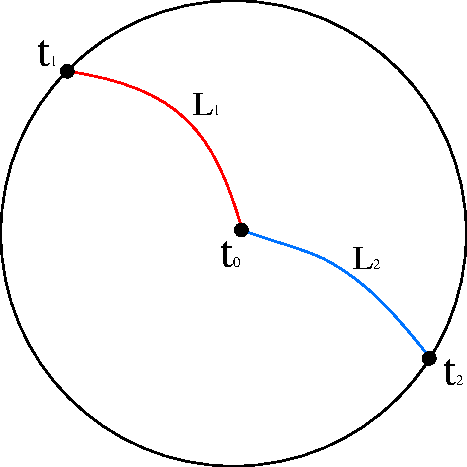
\includegraphics[width=0.7\linewidth]{graphics/scheme.pdf}~\\[15pt]\label{fig:TofSketch}\caption{Sketch of the exclusive event with two opposite-sign tracks in the magnetic field of the STAR Time Projection Chamber.\vspace{12pt}}
\end{minipage}
\hspace{0.1cm}
\begin{minipage}[b]{0.55\linewidth}
\centering
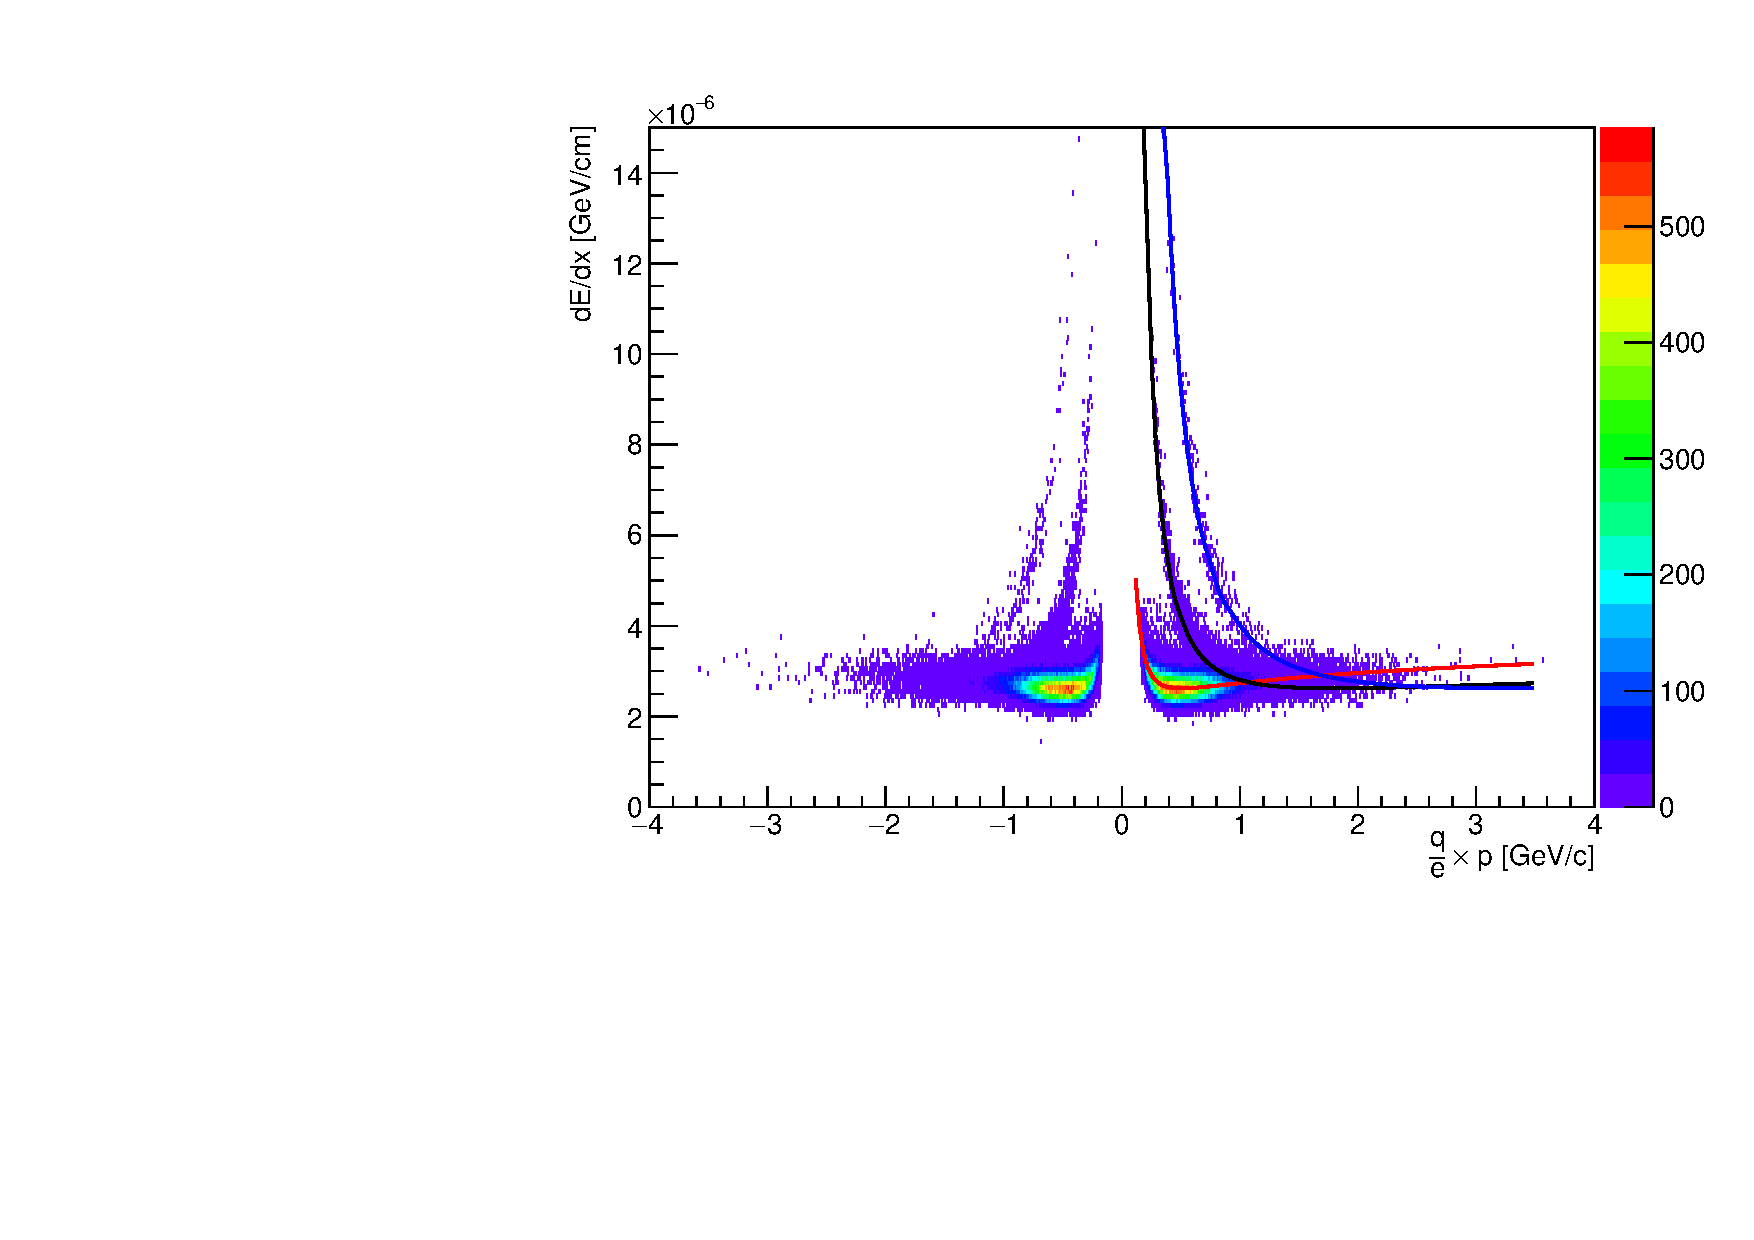
\includegraphics[width=\linewidth]{graphics/TestOfDEdxParametrisation.pdf}\label{fig:dEdx}\caption{Particle energy loss in TPC, dE/dx, as a function of charged particle momentum (STAR data). Colored lines depict dE/dx parametrisation, which agree well with the data.}
\end{minipage}
\end{figure}

Having defined such variables for both tracks, we form the measure of probability that a pair of tracks is of the same type $Y$:
\begin{equation}\label{eq:nSigmaPair}
 n\sigma_{Y}^{\text{pair}} = \sqrt{\left(n\sigma_{Y}^{\text{trk1}}\right)^{2} + \left(n\sigma_{Y}^{\text{trk2}}\right)^{2}}.
\end{equation}

In addition to information from the TPC we use time of hit detection in the barrel TOF subsystem. From the simple algebra describing relation between track lengths, momenta and times of hit detection one can derive formula for the squared mass of two particles, assuming that their masses are equal (particles are of the same type):

\begin{equation}
 \left\{\begin{array}{l}%
 t_{1}-t_{0} = L_{1}\sqrt{1+\frac{m_{1}^{2}}{p_{1}^{2}}}, \\[3pt]
 t_{2}-t_{0} = L_{2}\sqrt{1+\frac{m_{2}^{2}}{p_{2}^{2}}},
\end{array}\right.%
\end{equation}

\begin{equation}
 \Delta t = t_{1}-t_{2} = L_{1}\sqrt{1+\frac{m_{1}^{2}}{p_{1}^{2}}} - L_{2}\sqrt{1+\frac{m_{2}^{2}}{p_{2}^{2}}}.
\end{equation}

\[\textrm{Assuming}~m_{1}=m_{2}=m~~\rightarrow~~m^{2}~\textrm{from quadratic eq.}\]
Parameters of the quadratic equation whose solution is suqared mass and the final formula for $m^{2}_{\text{TOF}}$ are given below:
\begin{equation}
a= -2\frac{L^2_1L^2_2}{p^2_1p^2_2}+\frac{L^4_1}{p^4_1}+\frac{L^4_2}{p^4_2},
\end{equation}
\begin{equation}
b=-2L^2_1L^2_2\left({\frac{1}{p^2_1}} + {\frac{1}{p^2_2}}\right)+\frac{2L^4_1}{p_1^2}+\frac{2L^4_2}{p_2^2}-2\left(\Delta t\right)^2\left(\frac{L^2_1}{p_1^2}+\frac{L^2_2}{p_2^2}\right),
\end{equation}
\begin{equation}
c=\left(\Delta t\right)^4-2\left(\Delta t\right)^2\left(L^2_1+L^2_2\right)+L^4_1+L^4_2-2L^2_1L^2_2,
\end{equation}
\begin{equation}
 \label{eq:mSquared}
m^{2}_{\text{TOF}} = \frac{-b+\sqrt{b^2-4ac}}{2a}.
\end{equation}


Using variables defined in Eq.~\ref{eq:nSigmaPair} and~\ref{eq:mSquared} we can now present the logic of the nominal PID algorithm:
\begin{center}
\textbf{~~~if} $n\sigma_{\text{pion}}^{\text{pair}}>3$ \textbf{\&} $n\sigma_{\text{kaon}}^{\text{pair}}>3$ \textbf{\&} $n\sigma_{\text{proton}}^{\text{pair}}<3$ \textbf{\&} $m^{2}_{\text{TOF}}\in(0.7,1.1)~~~~~\rightarrow \textcolor{blue}{pp}$\\
~~~~\textbf{elif} $n\sigma_{\text{pion}}^{\text{pair}}>3$ \textbf{\&} $n\sigma_{\text{kaon}}^{\text{pair}}<3$ \textbf{\&} $n\sigma_{\text{proton}}^{\text{pair}}>3$ \textbf{\&} $m^{2}_{\text{TOF}}\in(0.2,0.32)~~~\rightarrow \textcolor{dgreen}{KK}$\\
~~~\textbf{elif} $|n\sigma_{\text{pion}}^{\text{trk1}}|<3$ \textbf{\&} $|n\sigma_{\text{pion}}^{\text{trk2}}|<3 ~~~~~~~~~~~~~~~~~~~~~~~~~~~~~~~~~~~~~~~~~~~~~~~~~~ \rightarrow \textcolor{red}{\pi\pi}~$\\
~~~\textbf{else}~~\textrm{PID fails} ~~~~~~~~~~~~~~~~~~~~~~~~~~~~~~~~~~~~~~~~~~~~~~~~~~~~~~~~~~~~~~~~~~~~~~~~~~~~~~~~~~ 
\end{center}



\section{Implementation}

Created software consists of the following files:\vspace*{-7pt}
\begin{enumerate}
\item Main.py - main program file\vspace*{-7pt}
\item EventGenerator.py - class generating exclusive events\vspace*{-7pt}
\item EventReconstruction.py - class transforming true-level data to detector-level\vspace*{-7pt}
\item ExclusiveEvent.py - class representing exclusive event\vspace*{-7pt}
\item ParticleId.py - class representing type of the particle (of an exclusive pair)\vspace*{-7pt}
\item StarDetectorAcceptance.py - class containing information about STAR detector acceptance\vspace*{-7pt}
\item TrackingSimulation.py - class performing track propagation in the STAR magnetic field\vspace*{-7pt}
\item dEdxParametrisation.py - class providing Bichsel parametrisation of dE/dx in the STAR TPC\vspace*{-7pt}
\item PlottingHistograms.py - class for histograms plotting
\end{enumerate}

Program executes a loop with a customizable number of iterations. In each loop one event is simulated, which starts from determination of the type of particles in a pair ($\pi\pi$, $KK$ or $pp$) according to the particle yields extracted from the STAR data. Then momenta of particles are read from the input files, which contain output of the GenEx generator~\cite{3} which provide momenta of exclusively produced particle pairs according to the Lebiedowicz-Szczurek model~\cite{4}. Particles are checked whether they fit in the STAR acceptance - if not, new set of momenta is read until they fulfill acceptance limitations. Particles are then tracked in the magnetic field of the STAR main detector using Newton's method. From this one obtains positions of the TOF module hit by the particles and thus one is able to recontruct the length of the tracks from the vertex to the TOF modules. Next, time of hits detection in TOF are reconstructed, and appropriate timing resolution of 100~ps is accounted. After all necessary quantities are known, dE/dx of both tracks are simulated using Bichsel parametrisation of the TPC response, and finally nSigma variables and $m^{2}_{\textrm{TOF}}$ are calculated in the very same way as the real data.
For every event PID algorithm is used to determine particle types, which are compared with true-level PID. Also histograms of many other quantities are filled and draw at the end of program execution.


\section{Program usage}
\begin{enumerate}
\item Download code from the GitHub repository~\cite{1}\vspace*{-7pt}
\item Set number of events to simulate and analyse in Main.py\vspace*{-7pt}
\item Start program with a standard command\\ \textit{:$\sim$\$ python Main.py}\vspace*{-7pt}
\item Once program execution is done you shall find output files in the Output directory.
\end{enumerate}
% One can easily change parameters of the program e.g. signal shape, noise levels etc. in file FitBox.py.





\section{Results}\vspace{-10pt}
\begin{figure}[ht]
\begin{minipage}[b]{0.55\linewidth}
\centering
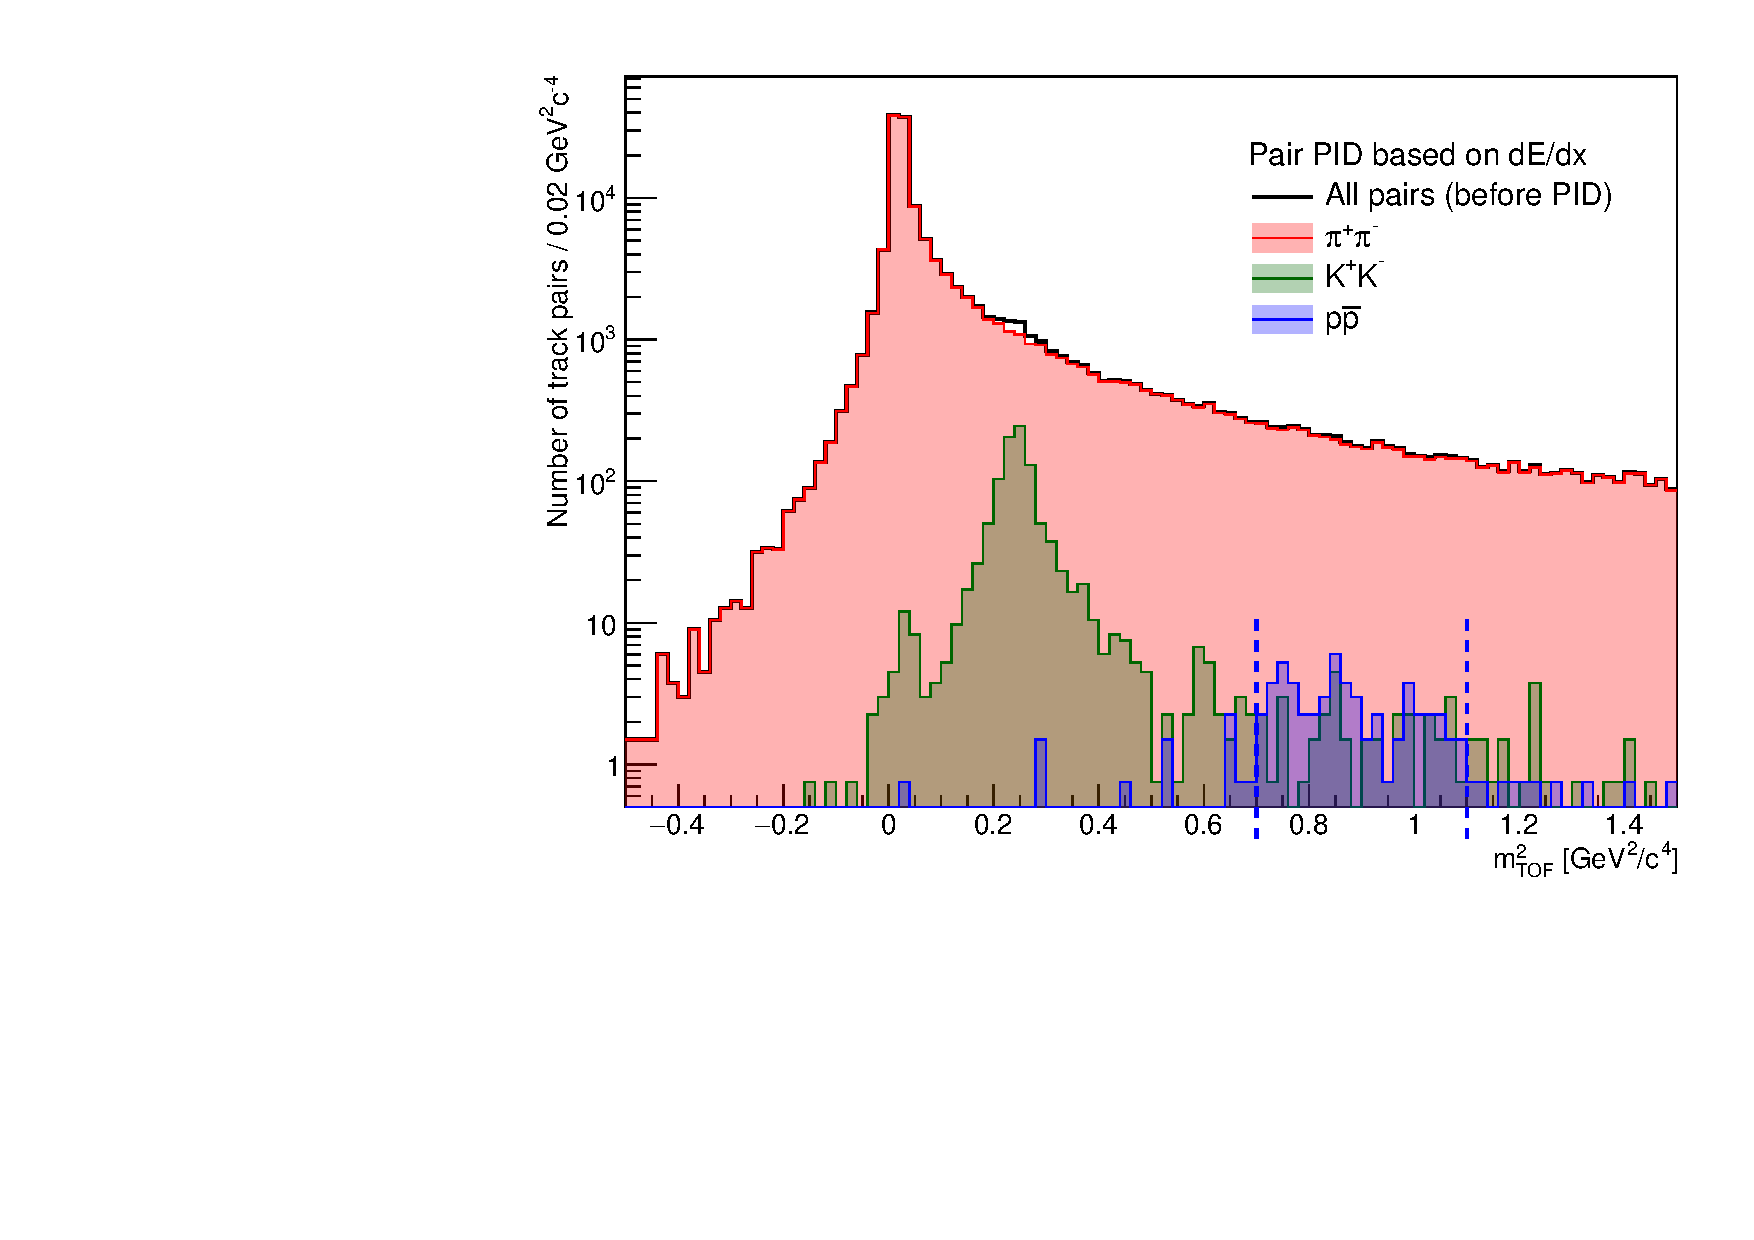
\includegraphics[width=\linewidth]{graphics/sqMassFromTof.pdf}\label{fig:mSquared}\caption{Squared mass $m^{2}_{\text{TOF}}$ (using Eq.~\ref{eq:mSquared}) in the desceribed PID procedure.}
\end{minipage}
\hspace{0.1cm}
\begin{minipage}[b]{0.44\linewidth}
\centering
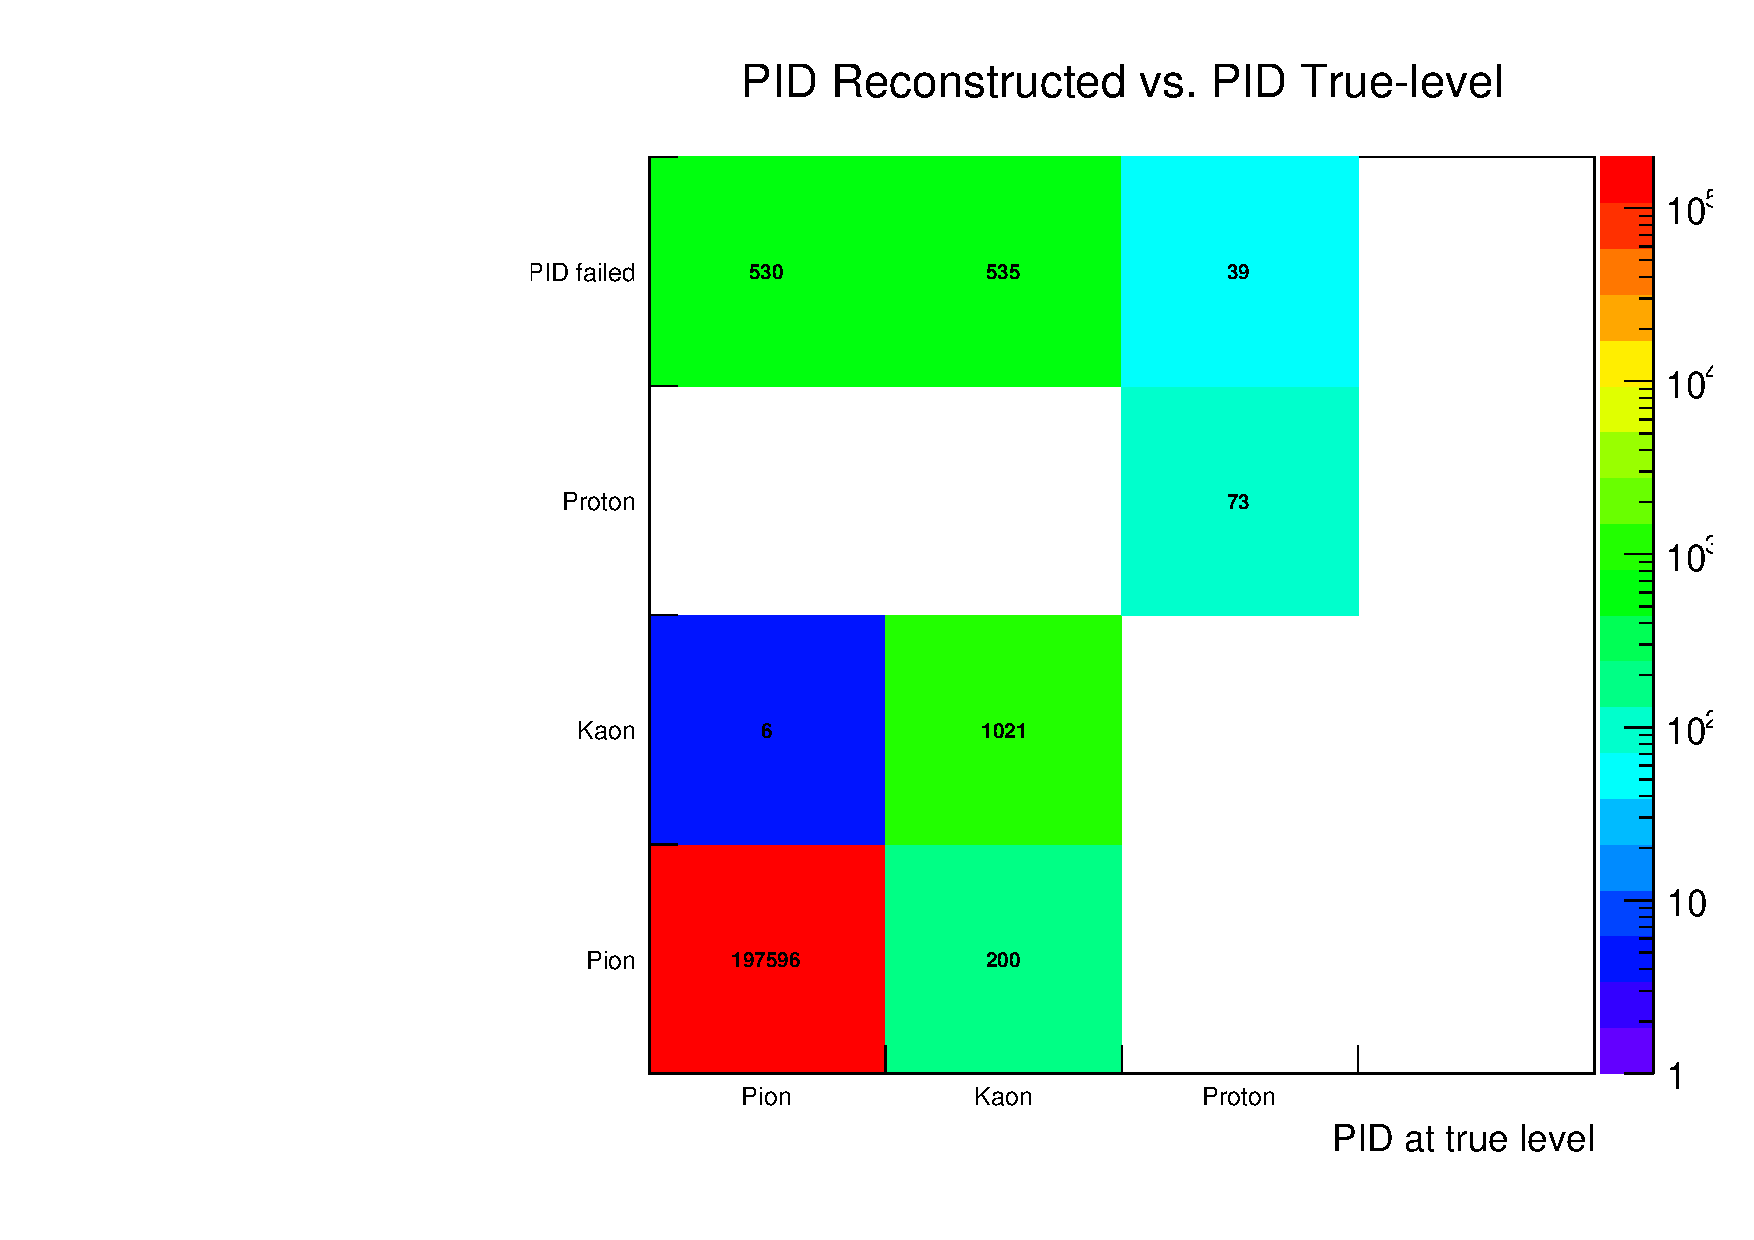
\includegraphics[width=\linewidth]{graphics/PidEfficiency.pdf}\label{fig:PID}\caption{Response matrix of the PID algorithm described in the text.}
\end{minipage}
\end{figure}

\begin{equation}\label{eq:eff}
 \textrm{Efficiency} = \epsilon = \frac{\textrm{number of XX pairs at true-level identified as XX}}{\textrm{number of XX pairs at true-level}}
\end{equation}
\begin{equation}\label{eq:pur}
 \textrm{Purity} = \psi = \frac{\textrm{number of XX pairs at true-level identified as XX}}{\textrm{number of pairs identified as XX}}
\end{equation}

\begin{table}[hb]
\centering
\begin{tabular}{c|C{2.9cm}|C{2.9cm}}
 & Efficiency $\epsilon$ & Purity $\psi$ \\ \hline
$\pi^{+}\pi^{-}$ & 99.7\% & 99.9\% \\ %\hline
$K^{+}K^{-}$ & 58.1\% & 99.4\% \\ %\hline
$p\bar{p}$ & 65.2\% & 100.0\% \\ %\hline
\end{tabular}
\caption{Efficiency and purity calculated based on simulation results depicted in Fig.~\ref{fig:PID} using Eqs.~\ref{eq:eff} and \ref{eq:pur}.}\label{tab:EfficiencyAndPurity}
\end{table}


\vspace{-10pt}
\begin{thebibliography}{0}
\bibitem{1} M.Shao \textit{et~al.}, \textit{Extensive particle identification with TPC and TOF at the STAR experiment}, Nucl. Instrum. Meth. \textbf{A558} (2006), 419-429, \href{http://arxiv.org/abs/nucl-ex/0505026}{arXiv:nucl-ex/0505026}.
\bibitem{2} \url{https://github.com/rafalsikora/PITE_PidForSTAR}
\bibitem{3} R.A.~Kycia, J.~Chwastowski, R.~Staszewski and J.~Turnau, \textit{GenEx: A simple generator structure for exclusive processes in high energy collisions}, \href{http://arxiv.org/abs/arXiv:1411.6035}{arXiv:1411.6035 [hep-ph]}.
\bibitem{4} P.Lebiedowicz and A.Szczurek, \textit{Revised model of absorption corrections for the $p p \to p p \pi^{+} \pi^{-}$ process}, Phys.Rev. \textbf{D92} (2015) no.5, 054001, \href{http://arxiv.org/abs/arXiv:1504.07560}{arXiv:1504.07560 [hep-ph]}.
\end{thebibliography}


\end{document}          
